\documentclass[%
 reprint,
%superscriptaddress,
%groupedaddress,
%unsortedaddress,
%runinaddress,
%frontmatterverbose, 
%preprint,
%showpacs,preprintnumbers,
%nofootinbib,
%nobibnotes,
%bibnotes,
 amsmath,amssymb,
 aps,
%pra,
%prb,
%rmp,
%prstab,
%prstper,
%floatfix,
]{revtex4-1}

\usepackage{graphicx}% Include figure files
\usepackage{caption}
\usepackage{subcaption}
\usepackage{dcolumn}% Align table columns on decimal point
\usepackage{bm}% bold math
\usepackage{hyperref}% add hypertext capabilities
\usepackage[mathlines]{lineno}% Enable numbering of text and display math
\usepackage{lipsum}
\usepackage{amssymb}
%\usepackage{subfigure}
%\usepackage{subfig}
%\linenumbers\relax % Commence numbering lines

%\usepackage[showframe,%Uncomment any one of the following lines to test 
%%scale=0.7, marginratio={1:1, 2:3}, ignoreall,% default settings
%%text={7in,10in},centering,
%%margin=1.5in,
%%total={6.5in,8.75in}, top=1.2in, left=0.9in, includefoot,
%%height=10in,a5paper,hmargin={3cm,0.8in},
%]{geometry}

\begin{document}

\preprint{APS/123-QED}

\title{Something about quantum discord}% Force line breaks with \\
%\thanks{A footnote to the article title}%

\author{The list of authors}
%\altaffiliation[Also at ]{Physics Department, XYZ University.}%Lines break automatically or can be forced with \\
%\author{Second Author}%
%\email{Second.Author@institution.edu}
%\affiliation{%
%Authors' institution and/or address\\
%This line break forced with \textbackslash\textbackslash
%}%

%\collaboration{MUSO Collaboration}%\noaffiliation

%\author{Charlie Author}
%\homepage{http://www.Second.institution.edu/~Charlie.Author}
%\affiliation{
%Second institution and/or address\\
%This line break forced% with \\
%}%
%\affiliation{
%Third institution, the second for Charlie Author
%}%
%\author{Delta Author}
%\affiliation{%
%Authors' institution and/or address\\
%This line break forced with \textbackslash\textbackslash
%}%

%\collaboration{CLEO Collaboration}%\noaffiliation

\date{\today}% It is always \today, today,
             %  but any date may be explicitly specified

\begin{abstract}
Something about quantum discord: abstract goes here.
%\begin{description}
%\item[Usage]
%Secondary publications and information retrieval purposes.
%\item[PACS numbers]
%May be entered using the \verb+\pacs{#1}+ command.
%\item[Structure]
%You may use the \texttt{description} environment to structure your abstract;
%use the optional argument of the \verb+\item+ command to give the category of each item. 
%\end{description}
\end{abstract}

%\pacs{Valid PACS appear here}% PACS, the Physics and Astronomy
                             % Classification Scheme.
%\keywords{Suggested keywords}%Use showkeys class option if keyword
                              %display desired
\maketitle

%\tableofcontents

\section{Introduction}
\noindent \lipsum[1-2]

\section{Quantum discord: the definition}
\noindent Quantum information provides several ways to define an amount of correlation between two parties or among multiple parties. Theoretically and experimentally, of particular interest of correlation are concurrence and the Bell nonlocality. For a given density matrix of a mixed state of two qubits, concurrence gives the amount of an entanglement monotone, whereas the Bell nonlocality provides the measure of nonlocality. However, in spite of their usefulness, those definitions do not provide the most general measure of the amount of correlation in quantum systems. Olliver \textit{et al.} approached this issue from the perspective of information science and proposed the theory of quantum discord in 2001. There exist variant versions of quantum discord, which will be introduced and discussed in the following subsections, but the central idea is shared by every version of quantum discord: purely extract the quantumness of correlations for a given density matrix. 

\begin{figure}
        \centering
        \begin{subfigure}[b]{0.45\textwidth}
                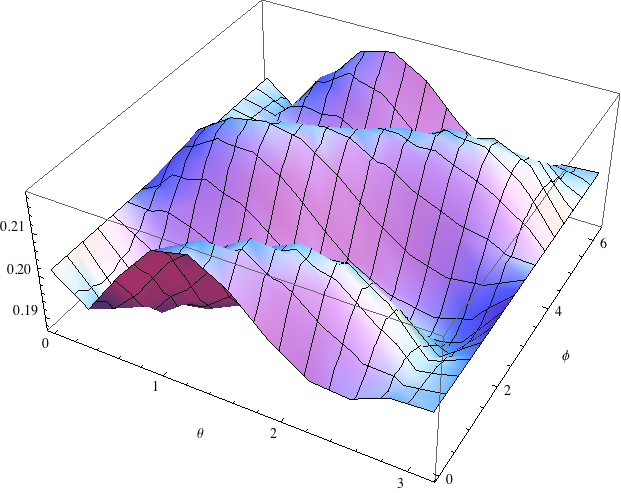
\includegraphics[width=\textwidth]{d}
                \caption{Entropic discord estimation of $\boldsymbol{\rho}_x$, varying $\theta$ and $\phi$.}
                \label{fig:ent.ex.}
        \end{subfigure}%
          %add desired spacing between images, e. g. ~, \quad, \qquad, \hfill etc.
          %(or a blank line to force the subfigure onto a new line)
        \vfill
        \begin{subfigure}[b]{0.45\textwidth}
                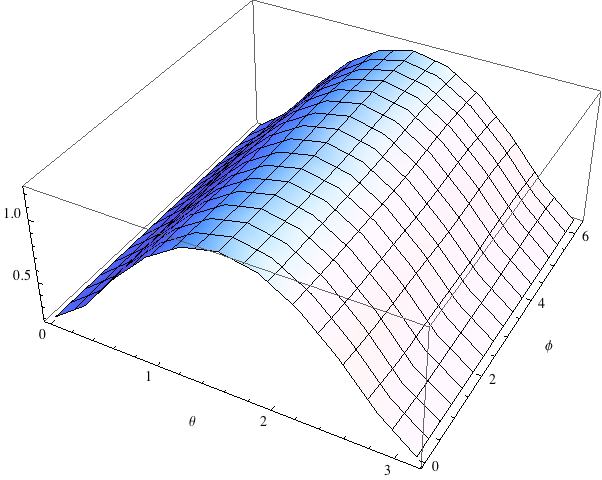
\includegraphics[width=\textwidth]{dg}
                \caption{Geometric discord estimation of $\boldsymbol{\rho}_x$, varying $\theta$ and $\phi$.}
                \label{fig:ent.ex.}
        \end{subfigure}%
        \caption{Entropic and geometric discord estimation of an arbitrary matrix $\boldsymbol{\rho}_x$.}\label{fig:ex.s}
\end{figure}

\subsection{Entropic discord}
\noindent For a classical system, information entropy or the Shannon entropy measures the ignorance about a discrete random variable $X$ with possible values $\{x_1, x_2, ..., x_n\}$. If the probability mass function is defined as $P(x_I)$, then the Shannon entropy is defined as follows:
\begin{equation}
H(X) = \sum_{i} P(x_i) I(x_i) = -\sum_{i} P(x_i) log_b P(x_i) \text{,}
\end{equation}
\noindent where $I$ is the information content of $X$, and b is the base of the logarithm used, commonly 2. Using the very definition of the Shannon entropy, we can find the mutual information of two random variables $A$ and $B$,
\begin{equation}
I(A:B) = H(A) + H(B) - H(A,B) \text{.}
\end{equation}

The quantum equivalence of information entropy and mutual information are similar to their classical counterparts. Quantum information entropy of a density matrix $\boldsymbol{\rho}$ is given by the famous von Neumann entropy, 
\begin{equation}
S(\boldsymbol{\rho}) = -tr(\boldsymbol{\rho} \  log_b \boldsymbol{\rho}) \text{.}
\end{equation}
\noindent Note that, for a qubit, $b=2$ since this normalizes the maximum entropic information of a qubit to 1. For a joint density matrix $\boldsymbol{\rho}_{AB}$, the mutual information $\textit{I}(\boldsymbol{\rho}_{AB})$ shared by quantum systems $A$ and $B$ is given by the following equation:
\begin{equation}
\textit{I}(\boldsymbol{\rho}_{AB}) = S(\boldsymbol{\rho}_A) + S(\boldsymbol{\rho}_B) - S(\boldsymbol{\rho}_{AB}) \label{quan.cor.} \text{,}
\end{equation}
\noindent where $\boldsymbol{\rho}_A$ ($\boldsymbol{\rho}_B$) can be deduced by the partial trace $tr_{B(A)} \  \boldsymbol{\rho}_{AB}$. However, this definition of mutual information embraces both the quantum mutual information and the classical mutual information. In order to get purely the quantumness of the correlation, namely quantum discord $\textit{D}(\boldsymbol{\rho}_{AB})$, one must need to deduct the classical measure of correlation $\textit{C}(\boldsymbol{\rho}_{AB})$ from the mutual quantum information $\textit{I}(\boldsymbol{\rho}_{AB})$:
\begin{equation}
\textit{D}(\boldsymbol{\rho}_{AB}) = \textit{I}(\boldsymbol{\rho}_{AB}) - \textit{C}(\boldsymbol{\rho}_{AB}) \text{.}
\end{equation}
\noindent The measure of classical correlation $\textit{C}(\boldsymbol{\rho}_{AB})$ is given by
\begin{equation}
\textit{C}(\boldsymbol{\rho}_{AB}) = \underset{\{B_k\}}{\text{sup}}\ \textit{I}(\boldsymbol{\rho}_{AB}|\{B_k\}) \label{clas.cor.} \text{,}
\end{equation}
\noindent where $\{B_k\}$ is a measurement performed locally on the system $B$. It is noteworthy that quantum discord is not generally symmetric under the exchange of the local system measurements. For instance, we can perform a set of measurements $\{A_k\}$, instead of $\{B_k\}$, and still have a equally valid measure of quantum discord. Note that Wu \textit{et al.} introduced \textit{symmetric discord} to ensure the symmetry. Nonetheless, this report follows the traditional definition of quantum discord, because the scope of interest generally considers the environment that has symmetric effects on the systems $A$ and $B$. An extensive discussion on how to perform the search algorithm for finding quantum discord is covered in the later section.

\subsection{Geometric discord}
\noindent Because we need to find the supremum of $\textit{I}(\boldsymbol{\rho}_{AB}|\{B_k\})$, the quantum discord between quantum systems $A$ and $B$ is not trivial to calculate. In fact, except for special classes of states such as two-qubit X density matrices, there does not exist a closed form solution for quantum discord, and as a consequence, one needs to implement complex numerical methods in order to calculate the quantumness of the correlation. 

In order to overcome this problem, Dakic \textit{et al.} and Tufarelli \textit{et al.} introduced geometric quantum discord that is based on the Hilbert-Schmidt distance between the density matrix $\boldsymbol{\rho}_{AB}$ and its closest classical state $\boldsymbol{\rho}_{AB}^{c}$, mathematically defined as
\begin{equation}
\textit{D}_G(\boldsymbol{\rho}_{AB}) = \underset{\{B_k\}}{\text{inf}}\  ||\boldsymbol{\rho}_{AB} - \boldsymbol{\rho}_{AB}^{c}||_{1}  \label{geom.} \text{,}
\end{equation}
\noindent where $||X||_{1}$ is the Hilbert-Schmidt 1-norm, defined as $||X||_{1} = tr(\sqrt{X^{\dagger}X})$. Note that, because $\boldsymbol{\rho}_{AB}^{c}$ is the closest classical state to $\boldsymbol{\rho}_{AB}$, it is also a zero quantum discord state, i.e. $\textit{D}(\boldsymbol{\rho}_{AB}^{c}) = 0$. This definition of quantum discord also requires numerical methods, but since there is no need to perform logarithms of matrices, the calculation process is simpler and faster, compared to the entropic definition of quantum discord.

There is another definition of geometric discord, based on the Hilbert-Schmidt 2-norm, 
\begin{equation}
\textit{D}_{G}^{(2)}(\boldsymbol{\rho}_{AB}) = \underset{\{B_k\}}{inf}\  ||\boldsymbol{\rho}_{AB} - \boldsymbol{\rho}_{AB}^{c}||_{2}^{2}  \text{,}
\end{equation}
\noindent where $||X||_{2} =\sqrt{tr(X^{\dagger}X)}$. However, recently it has been pointed out that the definition of geometric quantum discord based on the Hilbert-Schmidt 2-norm is not a good measure of quantum correlation, because it may increase under local reversible operations on the unmeasured subsystem. Hence, the discussion about the 2-norm definition will be omitted in this report. 

A extensive discussion on deriving zero quantum discord states and finding the infimum of the functional $||\boldsymbol{\rho}_{AB} - \boldsymbol{\rho}_{AB}^{c}||_{1}$ also comes in the following section.

\section{Numerical methods for quantum discord estimation}
\noindent This section discusses numerical methods to calculate two different definitions of quantum discord, entropic discord and geometric discord. For simplicity, the discussion starts with a general two-qubit density matrix, but the same algorithm can be applied to any multi-qudit systems. Note that the integrity of the algorithms described in the following are tested with numerous trials of randomly generated density matrices with known analytical solutions.

The estimation of entropic quantum discord consists of two parts. One part is to calculate $\textit{I}(\boldsymbol{\rho}_{AB})$ (eq. $\ref{quan.cor.}$), and it is fairly trivial. Note that $\boldsymbol{\rho}_{AB}$ is in the basis of $|i\rangle \otimes |j\rangle$ or $|ij\rangle$, where $i, j \in \{0, 1\}$. The other part is to find the supremum of the functional $\textit{I}(\boldsymbol{\rho}_{AB}|\{B_k\})$ (eq. $\ref{clas.cor.}$). Eq. $\ref{clas.cor.}$ can be expanded to a more explicit form, 
\begin{equation}
\textit{C}(\boldsymbol{\rho}_{AB}) = \underset{\{B_k\}}{\text{sup}} (S(\boldsymbol{\rho}_A) - S(\boldsymbol{\rho}_{AB}|\{B_k\})) \text{.}
\end{equation}
\noindent The second term in the equation is what requires a numerical approach. Let us define the second term as a function, 
\begin{equation}
\textit{F}(\boldsymbol{\rho}_{AB}) = \underset{\{B_k\}}{\text{inf}} S(\boldsymbol{\rho}_{AB}|\{B_k\}) \label{func.} \textit{.}
\end{equation}
\noindent The functional $S(\boldsymbol{\rho}_A|\{B_k\})$ is essentially a reduced density matrix of $A$, given the measurement $\{B_k\}$.

A qubit can have outcomes of either $|0\rangle$ or $|1\rangle$. However, any rotational transformation of $|0\rangle$ or $|1\rangle$ is a valid outcome of the measurement as well. For instance, we can define the polarization of light in the rectangular basis, but the diagonal basis is also equally valid. For this calculation, we need to consider all the possible measurement basis.

We start with two orthogonal measurement basis $\boldsymbol{\Pi}_0$ and $\boldsymbol{\Pi}_1$,
\begin{equation}
\boldsymbol{\Pi}_0 = 
\left( \begin{array}{cc}
1 & 0 \\
0 & 0 \end{array} \right) \text{, }
\boldsymbol{\Pi}_0 = 
\left( \begin{array}{cc}
0 & 0 \\
0 & 1 \end{array} \right) \text{.}
\end{equation}
\noindent By a simple rotational transformation $\textbf{V}$, we can generalize the measurement outcome $\{B_k\}$.
\begin{equation}
\textbf{V}(\theta,\phi) = \frac{1}{\sqrt{2}} (\textbf{I} - i \hat{a}^{\dagger}(\theta,\phi) \boldsymbol{\sigma} ) \text{,}
\end{equation}
\begin{equation}
\textbf{B}_k^i  = \textbf{V}^{\dagger} \boldsymbol{\Pi}_i \textbf{V} \text{, } i \in \{0, 1\} \text{.}
\end{equation}
\noindent Note that $\hat{a}$ is a unit vector in the Bloch sphere representation,
\begin{equation}
\hat{a}(\theta,\phi) = \left( \begin{array}{c}
sin \theta \  cos \phi \\
sin \theta \  sin \phi \\
cos \theta
\end{array} \right) \text{,}
\end{equation}
\noindent where $0 \le \theta \le \pi$ and $0 \le \phi \le 2\pi$. $\boldsymbol{\sigma}$ is a tensor of the Pauli matrices
\begin{equation}
\boldsymbol{\sigma} = \left( \begin{array}{c}
\boldsymbol{\sigma}_1 \\
\boldsymbol{\sigma}_2 \\
\boldsymbol{\sigma}_3
\end{array} \right) \text{,}
\end{equation}
\noindent and
\begin{eqnarray}
\boldsymbol{\sigma}_1 = \left( \begin{array}{cc}
0 & 1 \\
1 & 0
\end{array} \right) \text{, }
\boldsymbol{\sigma}_1 = \left( \begin{array}{cc}
0 & -i \\
i & 0
\end{array} \right) \text{, }
\boldsymbol{\sigma}_1 = \left( \begin{array}{cc}
1 & 0 \\
0 & -1
\end{array} \right) \text{. }
\end{eqnarray}

Using the above relations, we can deduce $\boldsymbol{\rho}_{AB}$ for a given set of measurement $\{B_k\}$,
\begin{equation}
\boldsymbol{\rho}_{AB|\{B_k\}} = \sum_{i \in \{0, 1\}} \frac{1}{p_i} (\textbf{I} \otimes \boldsymbol{B}_k^i) \boldsymbol{\rho}_{AB} (\textbf{I} \otimes \boldsymbol{B}_k^i) \text{,}
\end{equation}
\noindent where $p_i$ is given by $p_i = tr \{ (\textbf{I} \otimes \boldsymbol{B}_k^i) \boldsymbol{\rho}_{AB} (\textbf{I} \otimes \boldsymbol{B}_k^i) \}$. It is now obvious that the functional $\textit{S}(\boldsymbol{\rho}_AB|\{B_k\})$ of eq. $\ref{func.}$ is a function of $\theta$ and $\phi$, and we can numerically estimate the extremum by simply searching over the spherical space, $0 \le \theta \le \pi$ and $0 \le \phi \le 2\pi$.

Geometric quantum discord can be calculated in a similar manner. First, one needs to define an abtitrary zero quantum discord state for a given joint density matrix $\boldsymbol{\rho}_{AB}$. For this, let us define the reduced density matrix $\boldsymbol{\rho}_B$ given the measurement $|i\rangle$ of $A$, $i \in \{0, 1\}$, i.e. $\boldsymbol{\rho}_{B||0\rangle_A}$ and $\boldsymbol{\rho}_{B||1\rangle_A}$,
\begin{eqnarray}
\boldsymbol{\rho}_{B||0\rangle_A} = 
tr_A \left[ \left( \begin{array}{cc}
1 & 0 \\
0 & 0 \end{array} \right) \otimes
\boldsymbol{I} \right] \boldsymbol{\rho}_{AB} \text{,} \\
\boldsymbol{\rho}_{B||1\rangle_A} = 
tr_A \left[ \left( \begin{array}{cc}
0 & 0 \\
0 & 1 \end{array} \right) \otimes
\boldsymbol{I} \right] \boldsymbol{\rho}_{AB} \text{.}
\end{eqnarray}
\noindent Then, the zero quantum discord state $\boldsymbol{\rho}_{AB}^{c}$ can be found by using the following equation:
\begin{equation}
\boldsymbol{\rho}_{AB}^{c} = \sum_{i \in \{0,1\}} \left( \textbf{V}^{\dagger} \boldsymbol{\Pi}_i \textbf{V} \right) \otimes \boldsymbol{\rho}_{B||i\rangle_A} \text{.}
\end{equation}
\noindent Using the relations described above, eq. $\ref{geom.}$ can also be calculated by searching over the same spherical space, $0 \le \theta \le \pi$ and $0 \le \phi \le 2\pi$.

An example of entropic and geometric discord estimations, searching over the spherical space, $0 \le \theta \le \pi$ and $0 \le \phi \le 2\pi$, can be found in fig. $\ref{fig:ex.s}$. A random sample $\boldsymbol{\rho}_x$ is chosen for this demonstration:

$\boldsymbol{\rho}_x =$
\begin{align*}
\begin{small} \left( \begin{array}{cccc}
0.85 & 0.04 + 0.13 i & 0.01 + 0.01 i & 0.03 + 0.04 i \\
0.04 - 0.13 i & 0.07  & -0.02 + 0.04 i  & - 0.01 i \\
0.01 - 0.01 i & -0.02 - 0.04 i & 0.05 & 0.01 i \\
0.03 - 0.04 i & 0.01 i & - 0.01 i  & 0.03 \end{array} \right) \end{small}
\end{align*}
\noindent Both the entropic and the geometric discord values for the case $\boldsymbol{\rho}_x$ happen to be 0.19, though they are not usually identical. As observed, entropic discord can have multiple local minima which makes algorithmic optimization for quantum discord difficult. The geometric case in the figure looks monotonic, but in general it is not trivial to find the optimized approach as well.

\begin{figure}
        \centering
        \begin{subfigure}[b]{0.23\textwidth}
                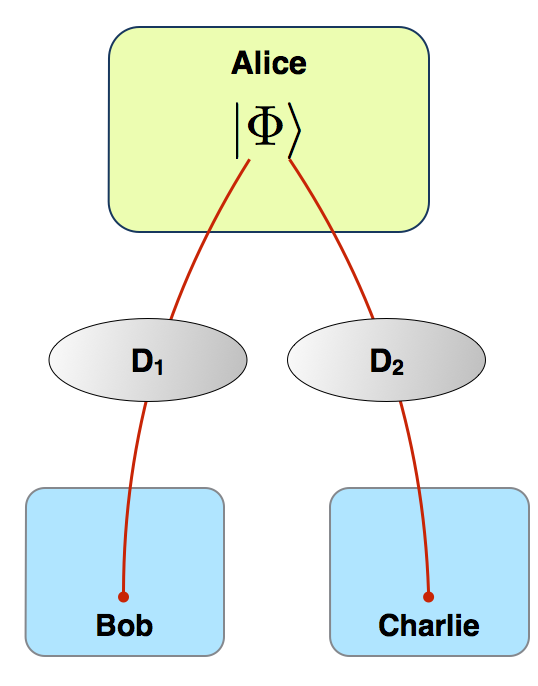
\includegraphics[width=\textwidth]{expd}
                \caption{}
                \label{fig:d}
        \end{subfigure}
        \begin{subfigure}[b]{0.23\textwidth}
                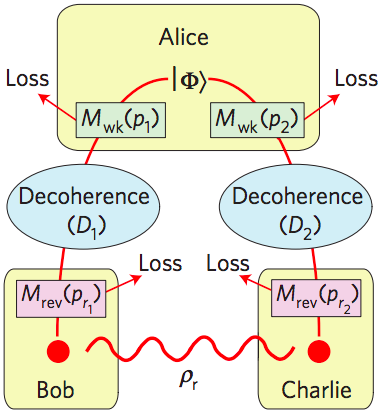
\includegraphics[width=\textwidth]{expw}
                \caption{}
                \label{fig:w}
        \end{subfigure}
        \caption{Scheme for protecting quantum correlation from decoherence using weak measurement and quantum measurement reversl, reprinted from Kim \textit{et al.}; a) Decoherence $D_1$ and $D_2$ in the quantum channels weaken the correlation of the joint quantum state $\rho_d$ between Bob and Charlie. b) such weakening can be reversed by sequential operations of weak measurement ($M_{wk}$) by Alice and reversing measurement ($M_{rev}$) by Bob and Charlie.}\label{fig:scheme}
\end{figure}

Although this brutal approach works fine, the optimization may be necessary for special cases. It is relatively easy to calculate the quantum discord of a two-qubit mixed state, but for qudits of $d>2$, search might take a very long time. As shown in fig. $\ref{fig:ex.s}$, one might encounter multiple local minima for a given arbitrary density matrix. Though we cannot yet rigorously prove which method of numerical estimation is the best way to deduce the quantum discord of an arbitrary quantum system, a number of numerical evaluations led us to the conclusion that the Monte Carlo sampling is sufficient for estimating the measure. Because it may be useful for calculating the quantum discord for a multi-qudit system, the general recipe is briefly discussed in the following.

For a qudit system, one can define the generalized Bloch sphere using the generalized Gell-Mann matrices, which are essentially the Pauli matrices equivalence of higher-dimensional extensions. For a qudit system of $N = d$, i.e. $SU(N)$, there are a total of $d^2-1$ Gell-Mann matrices. There are three classes: $\\$
i) $\frac{d(d-1)}{2}$ symmetric Gell-Mann matrices
\begin{equation} 
\Lambda_s^{jk} = |j\rangle \langle k|+|k\rangle \langle j|, 1 \le j < k \le d \text{,}
\end{equation}
ii) $\frac{d(d-1)}{2}$ antisymmetric Gell-Mann matrices
\begin{equation} 
\Lambda_a^{jk} = -i|j\rangle \langle k|+i |k\rangle \langle j|, 1 \le j < k \le d \text{,}
\end{equation}
iii) $(d-1)$ diagonal Gell-Mann matrices
\begin{equation} 
\Lambda_d^{l} = \sqrt{\frac{2}{l(l+1)}} \left(\sum_{j=1}^{l} |j\rangle \langle j|+ l|l+1\rangle \langle l+1| \right), 1 \le l \le d-1 \text{.}
\end{equation}
\noindent Using the Gell-Mann matrices, we can define the generalized Bloch vector expansion of a density matrix
\begin{equation}
\textbf{V} = \frac{1}{d} (\textbf{I}+\sqrt{d} \vec{b} \cdot \boldsymbol{\Lambda}) \text{,}
\end{equation}
\noindent where the Bloch vector $\vec{b} = (\{b^{jk}_s\}, \{b^{jk}_a\}, \{b^l\})$, and it consists of a total of $d^2-1$ components. If one uses a systemmatic approach to calculate quantum discord as described above, we can search over all the physical space span by $\vec{b}$, of which method consumes extensive computational resources. However, for the Monte Carlo sampling, each component in $\vec{b}$ is just a random variable. Programmatically speaking, we select $d^2-1$ random variables $\{\nu_1, \nu_2, ..., \nu_{d^2-1}\}$ and one additional random variable $r$, all uniformly distributed in the range from 0 to 1. With these random variables, we can construct $\vec{b}$ by the following way:
\begin{equation}
\vec{b} = \sqrt{\frac{r}{|\nu|^2}}(\{\nu_1, \nu_2, ..., \nu_{d^2-1}\}) \text{.}
\end{equation}
\noindent Using this construction, we can ensure $\vec{b} \in \mathbb{R}^{d^2-1}$, and by having $r$, we can cover all the possible Bloch vector, $|\vec{b}| \le 1$. Note that these randomly chosen density matrices must have physical values, i.e. Hermiticity or positive semidefiniteness. For instance, there is a possibility that diagonal terms of $\textbf{V}$ can be negative, if we carelessly applied the construction described above. One must be careful and eliminate such cases for calculation. The estimation method of the Monte Carlo sampling is tested under various cases, including two-qubit, two-qutrit cases, and more. Using this very method with a sufficiently large number of sampling can provide you a good estimation of quantum discord pretty quickly. The plots and figures are generated with all the methods described in this section, including the Monte Carlo sampling. 

\begin{figure}
        \centering
        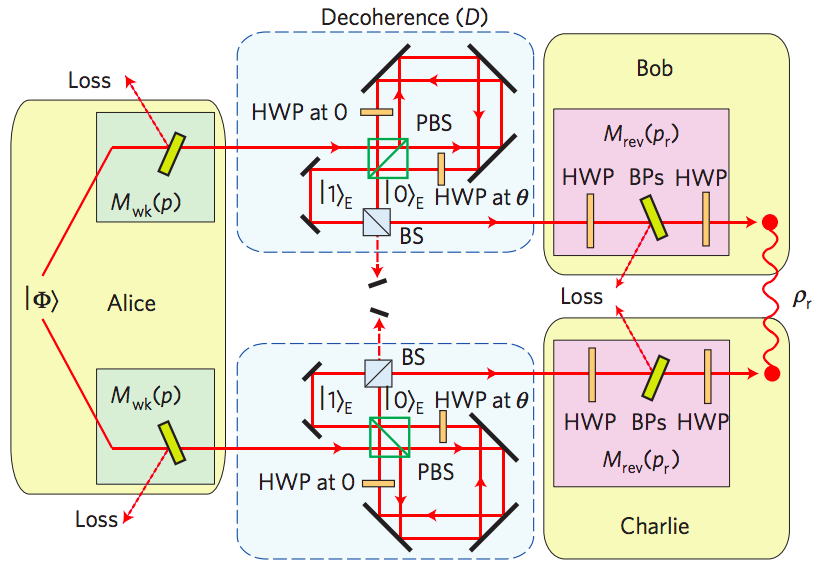
\includegraphics[width=0.49\textwidth]{setup}
        \caption{Schematic of the experiment, reprinted from Kim \textit{et al.}; The initial two-qubit state $|\Phi\rangle$ is prepared with the two-photon polarization state. $M_{wk}$ and $M_{rev}$ are performed with Brewster-angle glass plates (BPs) and half-wave plates (HWPs), respectively. We use an interferometer to simulate amplitude-damping decoherence.}\label{fig:setup}
\end{figure}

\section{Experiment}
\noindent The system of interest is a two-level system ($S$) whose computational bases are $\{|i\rangle_S\}$, where $i \in \{0,1\}$. Like any other quantum systems, this system also suffers from probabilistic and irreversible environmental decoherence or, for this particular model, amplitude-damping decoherence. We can model state-dependent coupling of the system S to the environment ($E$),
\begin{eqnarray}
|0\rangle_S \otimes |0\rangle_E  & \rightarrow & |0\rangle_S \otimes |0\rangle_E \text{,} \\
|1\rangle_S \otimes |0\rangle_E  & \rightarrow & \sqrt{\bar{D}} |1\rangle_S \otimes |0\rangle_E + \sqrt{D} |0\rangle_S \otimes |1\rangle_E \text{,}
\end{eqnarray}
\noindent where $0 \le D \le 1$ is the magnitude of the environmental decoherence and $\bar{D}=1-D$. Not only relevant to this particular case, amplitude-damping decoherence is a widely used model for various qubit systems, including examples such as zero-temperature energy relaxation for the superconducting qubit, photon loss for the vacuum single-photon qubit, and spontaneous decay for the atomic energy level qubit.

The experiment considers a quantum communication scenario depicted in the following, as shown in fig. $\ref{fig:scheme}$. Alice prepares a two-qubit correlated state $|\Phi\rangle$,
\begin{equation}
|\Phi\rangle = \alpha |00\rangle_S + \beta|11\rangle_S \text{,}
\end{equation}
\noindent where $|\alpha|^2+|\beta|^2=1$. This state is then delivered to Bob and Charlie through the quantum channels of which amplitude-damping decoherences are characterized as $D_1$ and $D_2$. The initially correlated state $|\Phi\rangle$ is then altered by the amplitude-damping decoherence effect, and the consequent two-qubit quantum state $\boldsymbol{\rho}_d$ in fig. $\ref{fig:d}$ shared by Bob and Charlie is now given as
\begin{align*}
\boldsymbol{\rho}_d =
\begin{small} \left( \begin{array}{cccc}
|\alpha|^2+D_1 D_2 |\beta|^2 & 0 & 0 & \sqrt{\bar{D}_1 \bar{D}_2} \alpha^* \beta \\
0 & D_1 \bar{D}_2 |\beta|^2 & 0 & 0 \\
0 & 0 & \bar{D}_1 D_2 |\beta|^2 & 0 \\
\sqrt{\bar{D}_1 \bar{D}_2} \alpha \beta^* & 0 & 0 & \bar{D}_1 \bar{D}_2 |\beta|^2 \end{array} \right) \end{small} \text{,}
\end{align*}
\noindent where $\bar{D}_k=1-D_k$, $k \in \{1,2\}$. Note that, in the absence of decoherence, $\textit{D}(\boldsymbol{\rho}_d) = \textit{D}_G(\boldsymbol{\rho}_d) = 1$. However, under the influence of maximal decoherence, i.e. $D_1=D_2=1$, $\textit{D}(\boldsymbol{\rho}_d) = \textit{D}_G(\boldsymbol{\rho}_d) = 0$.

We can make it turn around by sequential operations of weak measurement ($M_{wk}$) and reversing measurement ($M_{rev}$), performed beforehand and afterward of decoherence, respectively. These operations are non-unitary and defined as follows:
\begin{align*}
M_{wk} (p_1, p_2) &= \left( \begin{array}{cc}
1 & 0 \\
0 & \sqrt{1-p_1}
\end{array} \right) 
\otimes 
\left( \begin{array}{cc}
1 & 0 \\
0 & \sqrt{1-p_2}
\end{array} \right) \text{,} \\
M_{rev}(p_{r_1}, p_{r_2}) &= \left( \begin{array}{cc}
\sqrt{1-p_{r_1}} & 0 \\
0 & 1
\end{array} \right) 
\otimes 
\left( \begin{array}{cc}
\sqrt{1-p_{r_2}} & 0 \\
0 & 1
\end{array} \right) \text{,}
\end{align*}
\noindent where $p_i$ and $p_{r_i}$ are the strengths of the weak measurement and the reversing measurement for Bob ($i=1$) and Charlie ($i=2$), respectively. The optimal strength for the reversing measurement that maximizes the amount of correlation of the joint state $\boldsymbol{\rho}_r$ is $p_{r_i} = (1-D_i) p_i + D_i$. Assuming that the experiment is operating at the optimal weak and reversing measurements, the two-qubit state $\boldsymbol{\rho}_r$ in $\ref{fig:w}$ is now given as
\begin{align*}
\boldsymbol{\rho}_r = \frac{1}{\textit{A}}
\begin{small} \left( \begin{array}{cccc}
|\alpha|^2+\bar{p}_1 \bar{p}_2 D_1 D_2 |\beta|^2 & 0 & 0 & \alpha^* \beta \\
0 & \bar{p}_1 D_1 |\beta|^2 & 0 & 0 \\
0 & 0 & \bar{p}_2 D_2 |\beta|^2 & 0 \\
\alpha \beta^* & 0 & 0 & |\beta|^2 \end{array} \right) \end{small} \text{,}
\end{align*}
\noindent where $\textit{A} = 1+\{\bar{p}_1 D_1(1+\bar{p}_2 D_2)+\bar{p}_2 D_2\} |\beta|^2$ and $\bar{p}_i=1-p_i$.

The experimental setup is schematically shown in fig. $\ref{fig:setup}$, and you can find details in the section Methods of Kim $\textit{et al.}$ Note that, for the experimental demonstration, $D_1=D_2=D$ and $p_1=p_2=p$ are used, and the qubits are realized with the single-photon polarization state, where $|0\rangle$ and $|1\rangle$ are the horizontal and vertical polarizations, respectively.

\begin{figure}
        \centering
        \begin{subfigure}[b]{0.49\textwidth}
                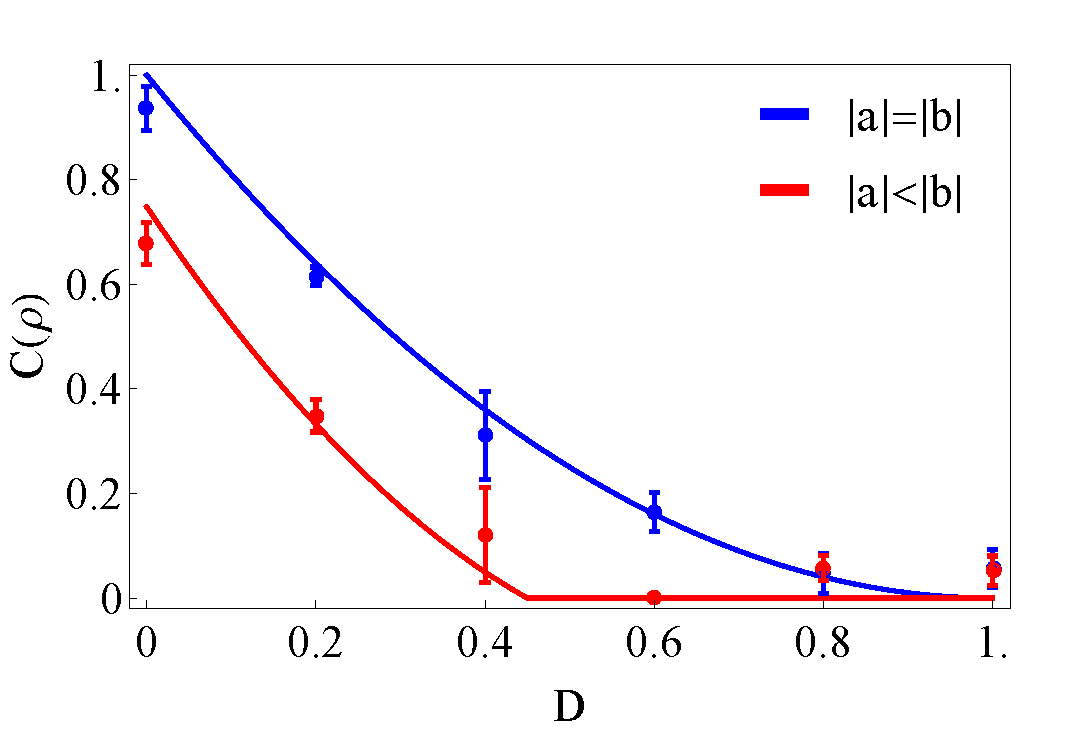
\includegraphics[width=\textwidth]{concd}
                \caption{}
                \label{fig:concd}
        \end{subfigure}
        \vfill
        \begin{subfigure}[b]{0.49\textwidth}
                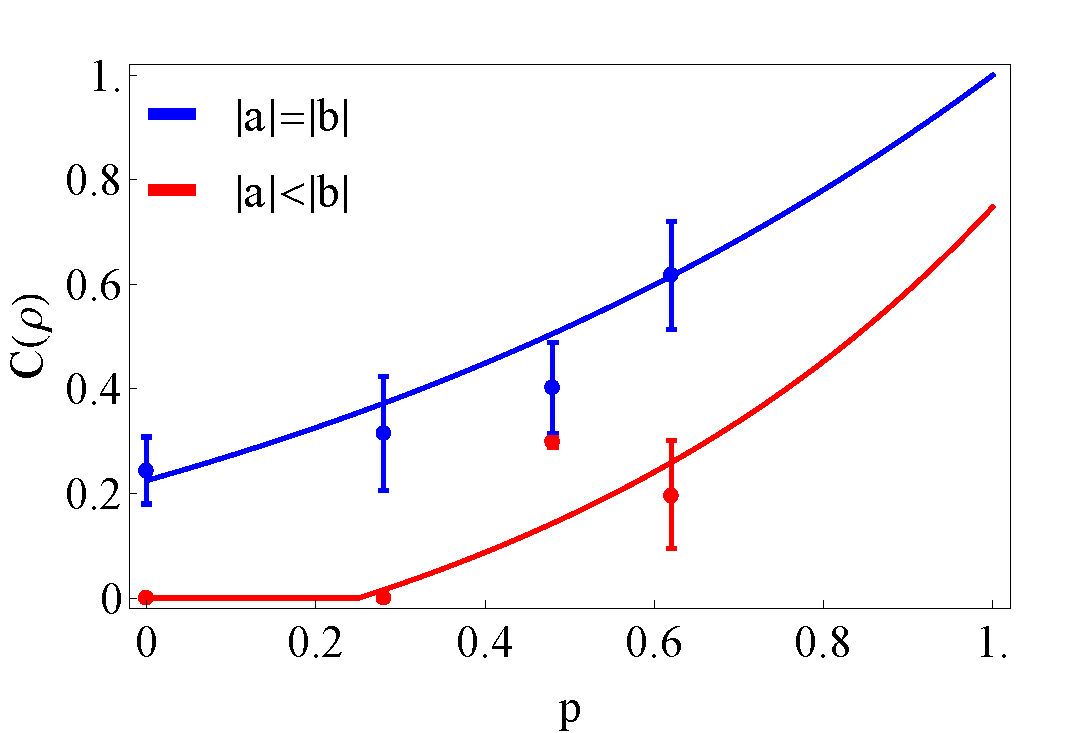
\includegraphics[width=\textwidth]{concw}
                \caption{}
                \label{fig:concw}
        \end{subfigure}
        \caption{Experimental data fitted to concurrence, reprinted from Kim \textit{et al.}; a) As D increases, the concurrence of $\boldsymbol{\rho}_d$ gradually decreases. b) Even under the influence of strong decoherence ($D=0.6$), we can revive the concurrence of $\boldsymbol{\rho}_r$ by $M_{wk}(p)$ and the corresponding optimal $M_{rev}(p_r)$.}\label{fig:conc}
\end{figure}

\subsection{A brief discussion of the concurrence result}
\noindent Concurrence defines the amount of entanglement monotone for a two-qubit mixed state,
\begin{equation}
\textit{C}(\boldsymbol{\rho}) = \text{max}(0, \lambda_1-\lambda_2-\lambda_3-\lambda_4) \text{.}
\end{equation}
\noindent $\lambda_1$, ..., $\lambda_4$ are the eigenvalues, in decreasing order, of the Hermitian matrix $R=\sqrt{\sqrt{\boldsymbol{\rho}}\tilde{\boldsymbol{\rho}}\sqrt{\boldsymbol{\rho}}}$, where $\tilde{\boldsymbol{\rho}} = (\sigma_2 \otimes \sigma_2)\boldsymbol{\rho}^* (\sigma_2 \otimes \sigma_2)$. The previous experiment presented in Kim \textit{et al.} was originally conducted to study the influence of decoherence and the effect of weak and reversing measurements on the concurrence. The result is reprinted from Kim \textit{et al.} and shown in fig. \ref{fig:conc}.

% Discuss the result briefly.

\subsection{Theoretical estimation of quantum discord under the same scenario}
\noindent In comparison with the original expriment by Kim \textit{et al.}, we examine how entropic discord ($\textit{D}(\boldsymbol{\rho})$) and geometric discord ($\textit{D}_G(\boldsymbol{\rho})$) behave under different decoherence, weak measurement, and the corresponding oprimal reversing measurement. In figs. $\ref{fig:A5}$ and $\ref{fig:A5G}$, we simulate the quantum discords for two particular initial states ($|\alpha|=|\beta|$ and $|\alpha|=0.42<|\beta|$). Similarly to the concurrence in fig. 4 of Kim $\textit{et al.}$, the plots clearly show that decoherence affects the two qubits independently, and their correlations can be circumvented by exploiting weak measurement and quantum measurement reversal. However, it is noteworthy that, for quantum discord, decoherence does not cause sudden death of correlation, unlike entanglement sudden death (ESD) for the concurrence case.

\begin{figure}
        \centering
        \begin{subfigure}[b]{0.23\textwidth}
                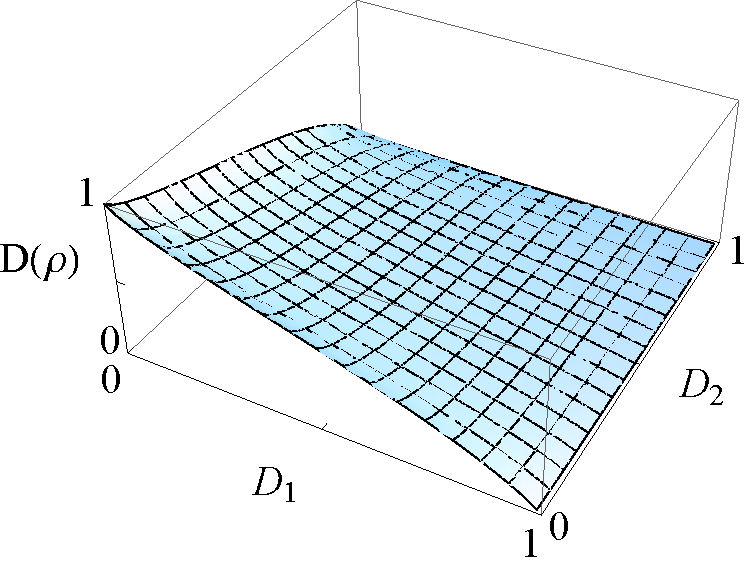
\includegraphics[width=\textwidth]{sq2D}
                \caption{}
                \label{fig:A1}
        \end{subfigure}
        \begin{subfigure}[b]{0.23\textwidth}
                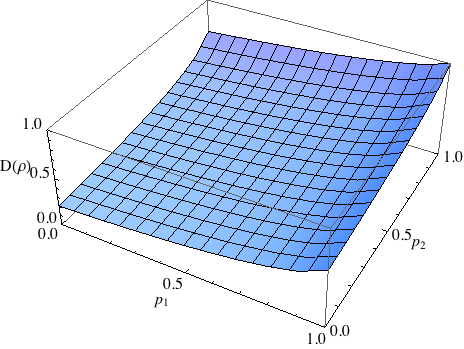
\includegraphics[width=\textwidth]{sq2W}
                \caption{}
                \label{fig:A2}
        \end{subfigure}
        \vfill
        \begin{subfigure}[b]{0.23\textwidth}
                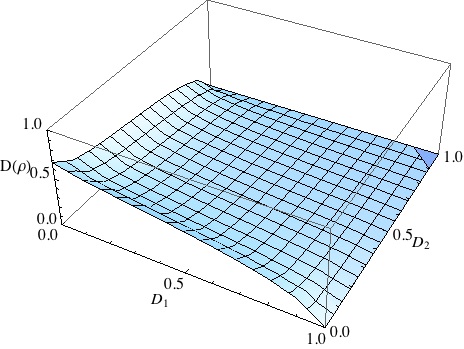
\includegraphics[width=\textwidth]{041D}
                \caption{}
                \label{fig:A3}
        \end{subfigure}
        \begin{subfigure}[b]{0.23\textwidth}
                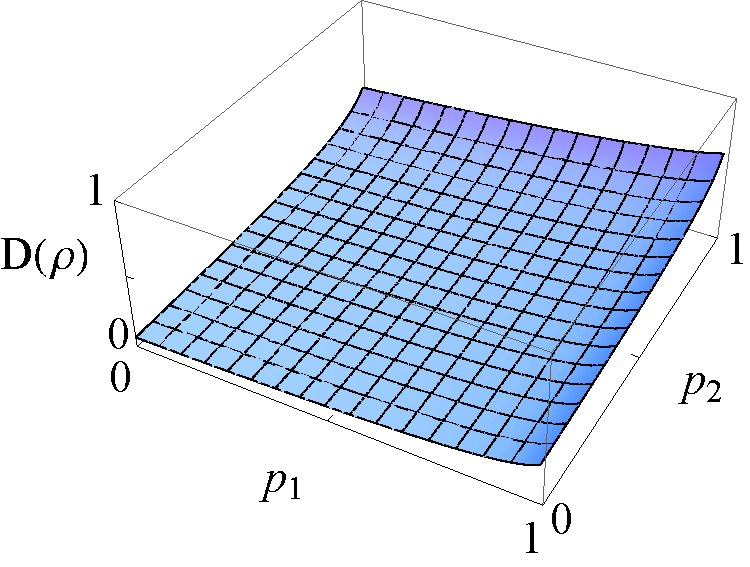
\includegraphics[width=\textwidth]{041W}
                \caption{}
                \label{fig:A4}
        \end{subfigure}
        \caption{Theoretical estimation of entropic discord as functions of decoherence and weak measurement; a) and b) are for the maximally correlated state $|\Phi\rangle$ with $|\alpha|=|\beta|$, and c) and d) are for the non-maximally correlated state $|\Phi\rangle$ with $|\alpha| < |\beta|$ with $\alpha=0.42$. Entropic quantum discord under the influence of decoherence is shown in a) and c), whereas the effect of the optimal weak and reversing measurements is shown in b) and d). Plots b) and d) are taken with $D_1 = 0.6$ and $D_2 = 0.8$.}\label{fig:A5}
\end{figure}

\begin{figure}
        \centering
        \begin{subfigure}[b]{0.23\textwidth}
                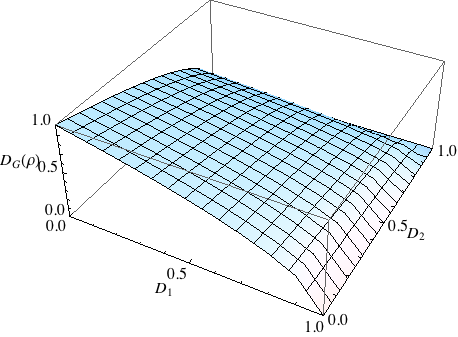
\includegraphics[width=\textwidth]{sq2DG}
                \caption{}
                \label{fig:A1G}
        \end{subfigure}
        \begin{subfigure}[b]{0.23\textwidth}
                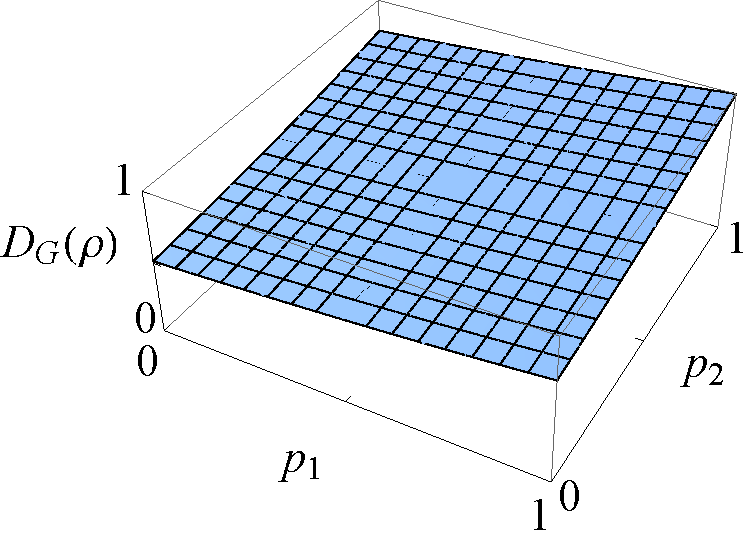
\includegraphics[width=\textwidth]{sq2WG}
                \caption{}
                \label{fig:A2G}
        \end{subfigure}
        \vfill
        \begin{subfigure}[b]{0.23\textwidth}
                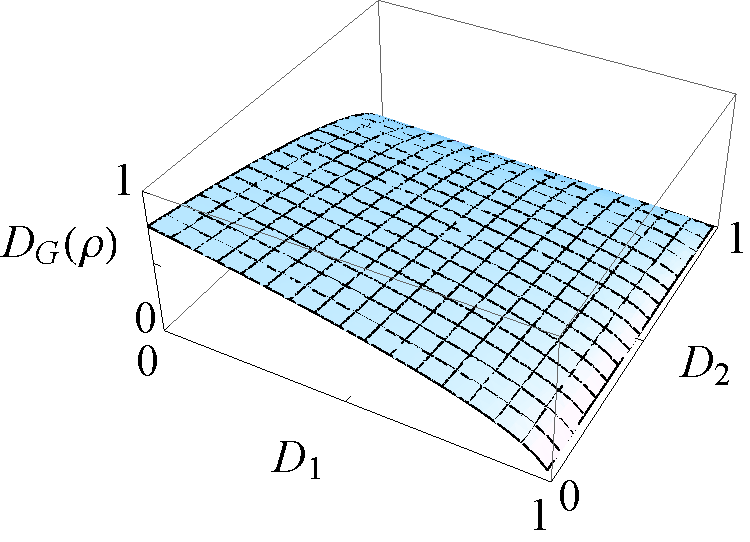
\includegraphics[width=\textwidth]{041DG}
                \caption{}
                \label{fig:A3G}
        \end{subfigure}
        \begin{subfigure}[b]{0.23\textwidth}
                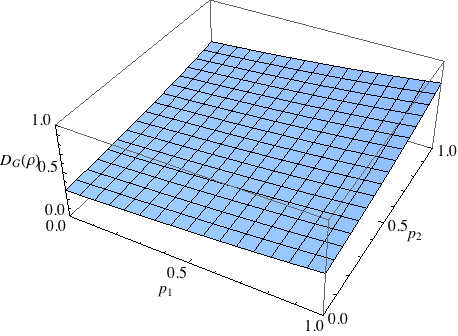
\includegraphics[width=\textwidth]{041WG}
                \caption{}
                \label{fig:A4G}
        \end{subfigure}
        \caption{Theoretical estimation of geometric discord as functions of decoherence and weak measurement; a) and b) are for the maximally correlated state $|\Phi\rangle$ with $|\alpha|=|\beta|$, and c) and d) are for the non-maximally correlated state $|\Phi\rangle$ with $|\alpha| < |\beta|$ with $\alpha=0.42$. Geometric quantum discord under the influence of decoherence is shown in a) and c), whereas the effect of the optimal weak and reversing measurements is shown in b) and d). Plots b) and d) are taken with $D_1 = 0.6$ and $D_2 = 0.8$.}\label{fig:A5G}
\end{figure}

\section{Result}
\begin{figure}
        \centering
        \begin{subfigure}[b]{0.49\textwidth}
                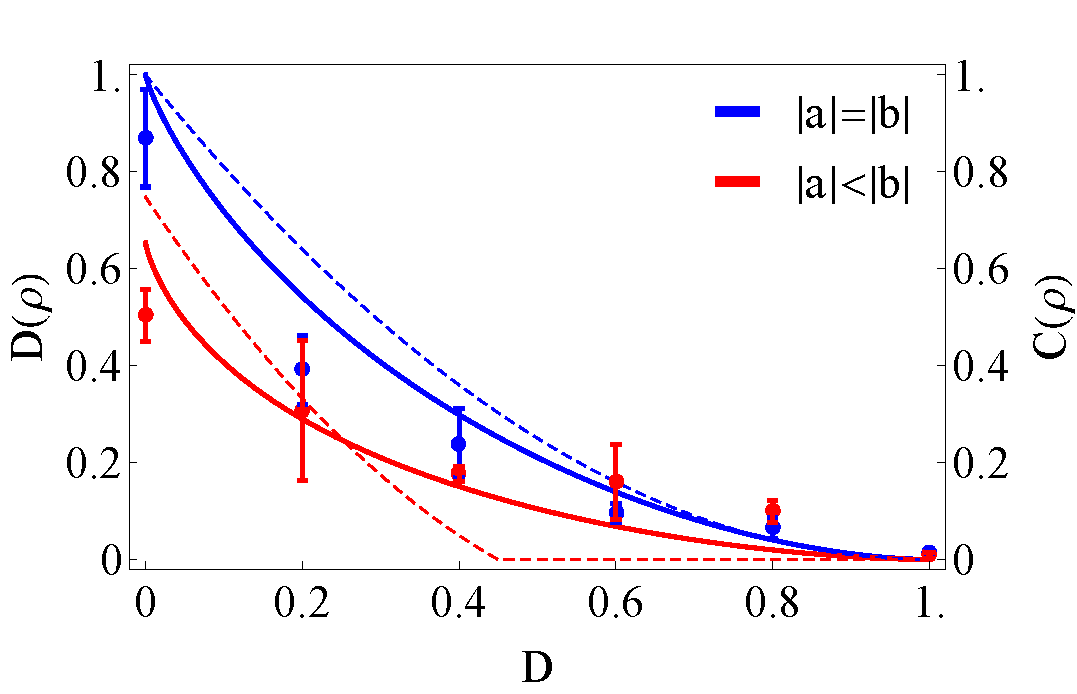
\includegraphics[width=\textwidth]{DD}
                \caption{}
                \label{fig:DD}
        \end{subfigure}
        \vfill
        \begin{subfigure}[b]{0.49\textwidth}
                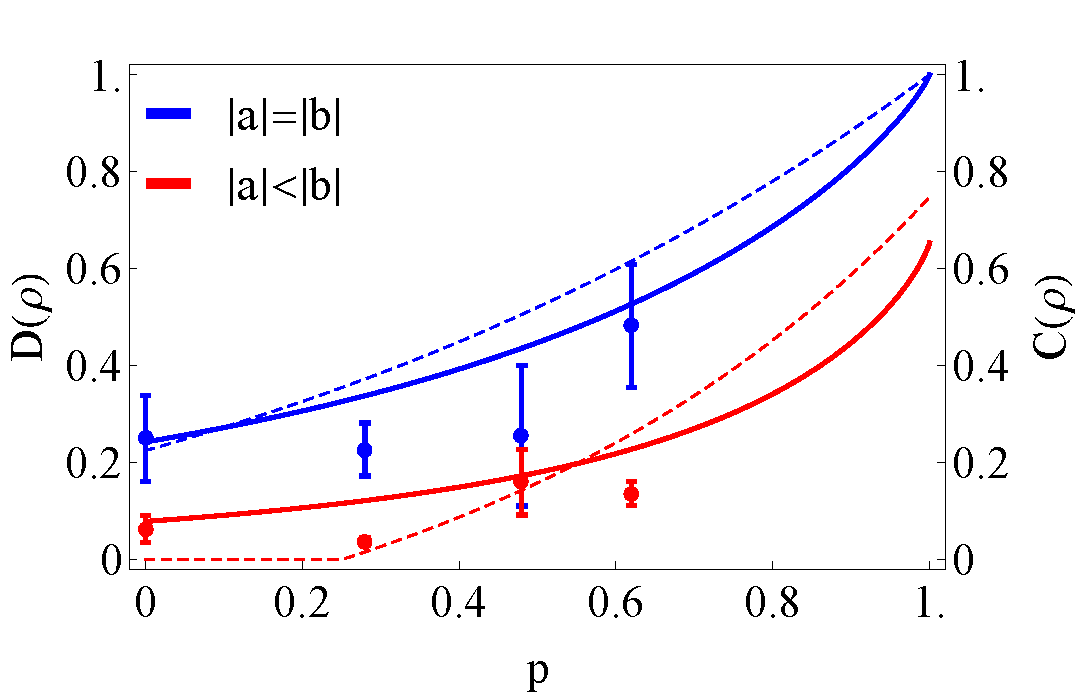
\includegraphics[width=\textwidth]{Dp}
                \caption{}
                \label{fig:Dp}
        \end{subfigure}
        \caption{Something.}\label{fig:D}
\end{figure}

\begin{figure}
        \centering
        \begin{subfigure}[b]{0.49\textwidth}
                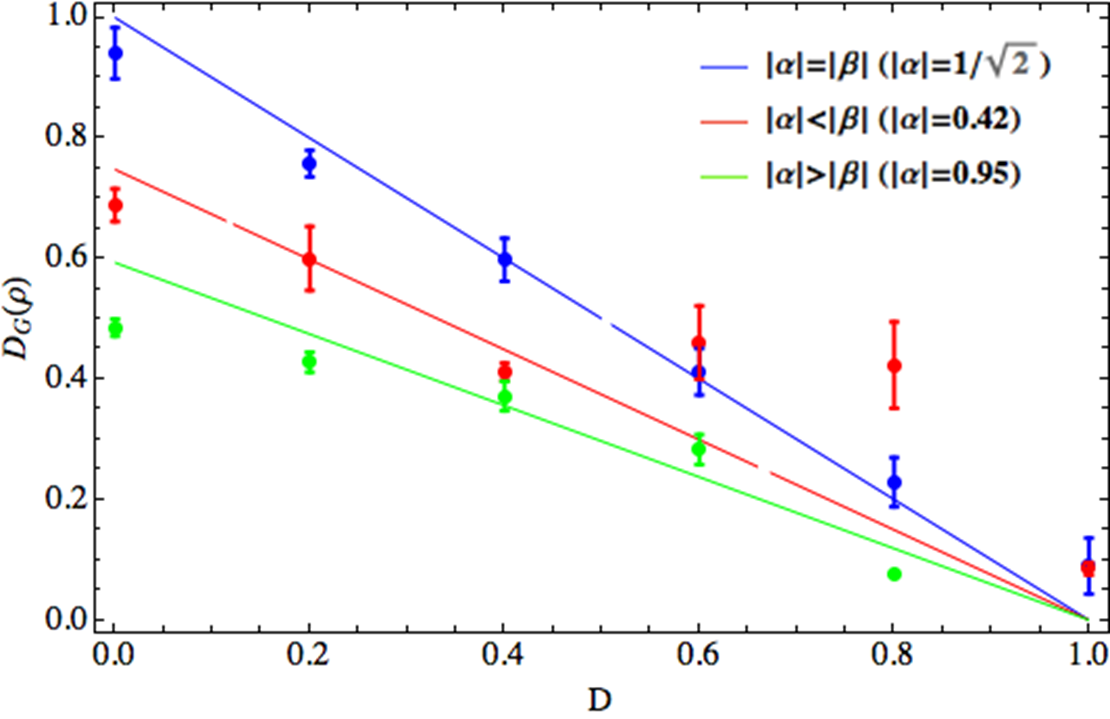
\includegraphics[width=\textwidth]{DGD}
                \caption{}
                \label{fig:DGD}
        \end{subfigure}
        \vfill
        \begin{subfigure}[b]{0.49\textwidth}
                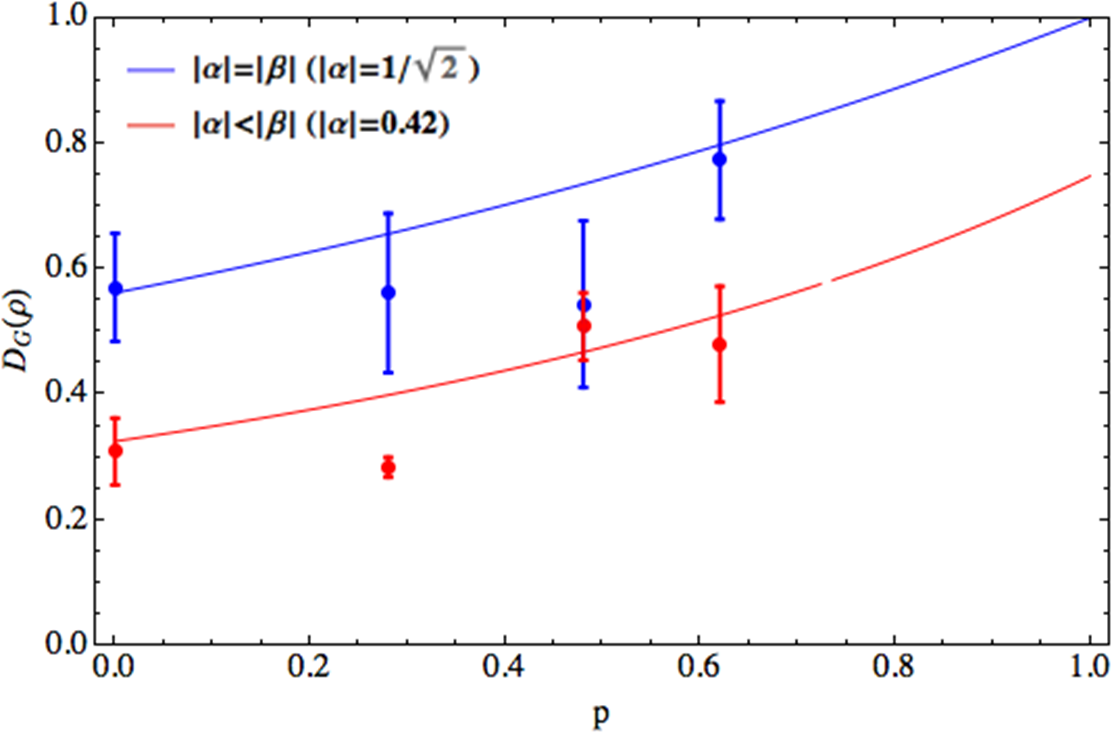
\includegraphics[width=\textwidth]{DGp}
                \caption{}
                \label{fig:DGp}
        \end{subfigure}
        \caption{Something.}\label{fig:DG}
\end{figure}

\noindent Experimentally, we first demonstrate the effect of decoherence $D$ on the initial two qubit mixed state $|\Phi\rangle = \alpha |00\rangle_S + \beta |11\rangle_S$. The measurement is performed with the setup described in fig. $\ref{fig:setup}$, and its two-qubit state $\boldsymbol{\rho}_d$ is recontructed with quantum state tomography. For the given $\boldsymbol{\rho}_d$, both entropic and geometric discord are evaluated. As shown in figs. $\ref{fig:DD}$ and $\ref{fig:DGD}$, we take data points for three input state conditions ($|\alpha|=|\beta|$, $|\alpha|<|\beta|$, and $|\alpha|>|\beta$) as a function of decoherence $D$.

As observed in the figures, unless the strength of decoherence is at its maximum, i.e. $D=1$, both the entropic and geometric discords between Bob and Charlie do not disappear. This is the most notable difference between quantum discord and concurrence. 

We also test whether the correlation between Bob and Charlie can be resurrected by weak measurement and quantum measurement reversal. The experimental conditions are the same as described in Kim $\textit{et al.}$ as well. The chosen decoherence parameter is set at $D=0.6$. Figs. $\ref{fig:Dp}$ and $\ref{fig:DGp}$ show the entropic and geometric discords of the two-qubit state $\boldsymbol{\rho}_r$, respectively, for two different sets of initial states: $|\alpha|=|\beta|$ and $|\alpha|<|\beta|$.

The reversing measurement parameter $p_r$ is optimally chosen such that $p_r=p(1-D)+D$ for a given weak measurement strength $p$. As shown in the figures $\ref{fig:D}$ and $\ref{fig:DG}$, the experiment shows that the sequential operations of weak measurement and reversing measurement can indeed suppress decoherence in quantum channels. Furthermore, under more optimized and ideal experimental conditions, we can even bring the amount of quantum discord to the level close to unity, as the weak measurement strength $p$ converges to 1.

\section{Discussion}
\noindent As Kim $\textit{et al.}$ already has shown with concurrence, we also have demonstrated that quantum correlation can be protected from decoherence by weak measurement and quantum measurement reversal. For this particular experiment in the scenario of amplitude-damping decoherence, we have proved that this protocol can be used for protecting quantum correlation from severe decoherence, and hence, enables the distribution of correlated quantum resources through quantum channels even under the influence of decoherence.

Furthermore, the protocol described in this paper can be applied to other types of quantum system beyond two-photon polarization qubits. For instance, there have been multiples studies done on quantum discord of Gaussian states. Under any scenarios, we believe that this protocol is a compelling method that can be used for effectively handling decoherence and distilling quantum correlations from decohered quantum resources. 

\section{References}
\lipsum[1-3]

\end{document}

%
%
%
%
%
%
%
%
%
%
%
%
%
%
%
%
%
%
%
%
%
%
%
%
%
%
%
%
%
%
%
%
%
%
%
